\documentclass[main.tex]{subfiles}

\begin{document}
  % ----------------------------------------------------------------------------
  % ------------------------------ Section 13 ----------------------------------
  % ----------------------------------------------------------------------------
  \section{Tétel – Az operációs rendszerek alapjai} %13
  
  \fogalom{Az operációs rendszer céljai, feladatai}
  Az \zkod{operációs rendszer} egy programrendszer,
  mely közvetítő szerepet lát el a számítógép felhasználója
  és a számítógép hardvere között.
  
  \vspace{1em}
  {\large \zkod{Céljai}:}
  \begin{itemize}
    \item felhasználói programok végrehajtása,
    felhasználói feladatmegoldás megkönnyítése

    \item a számítógép rendszer használatának
    megkönnyítése

    \item a számítógép hardver kihasználásának
    áhatékonyabbá tétele
  \end{itemize}

  {\large \zkod{Számítógép rendszerek komponensei}:}
  \begin{itemize}
    \item \zkod{hardver}: az alapvető számítási erőforrásokat nyújtja
    \item \zkod{operációs rendszer}: koordinálja és vezérli
    a hardver erőforrások különböző felhasználók különböző
    által történő használatát
    \item \zkod{alkalmazói programok}: definiáljá azt a módot,
    ahogyan az egyes rendszer-erőforrásokat a felhasználók
    számítási problémáinak megoldásához fel kell használni.
    (fordítók, adatbázis kezelők, videó játékok, ügyviteli programok)
    \item \zkod{felhasználók}: emberek, gépek, más számítógépek
  \end{itemize}

  {\large \zkod{Komponensei}:}
  \vspace{1em}

  \begin{minipage}[t]{0.5\textwidth}
    \begin{itemize}
      \item folyamat kezelés
      \item másdlagos tár kezelés
      \item fájl kezelés
      \item hálózat-elérés támogatása
    \end{itemize}
  \end{minipage}\hfill
  \begin{minipage}[t]{0.5\textwidth}
    \begin{itemize}
      \item memória gazdálkodás
      \item \zkod{IO} rendszer kezelés
      \item védelmi rendszer
      \item parancs-interpreter rendszer
    \end{itemize}
  \end{minipage}\hfill
  

  \fogalom{Folyamatok kommunikációja}

  A folyamat (\zkod{process}) egy végrehajtás alatt lévő program.
  Bizonyos erőforrásra van szüksége, hogy feladatát megoldhassa.
  (\zkod{CPU}, memória, állományok, \zkod{IO} berendezések)
  Az operációs rendszer az alábbi tevékenységekért felel:
  \begin{itemize}
    \item folyamat létrehozása/törlése
    \item folyamat felfüggesztése/újraindítása
    \item eszközök biztosítása
    (folyamatok szinkronizációjához, kommunikációjához)
  \end{itemize}
  A folyamat a multiprogramozott operációs rendszerek alapfogalma.
  A folyamaton általában műveletek meghatározott sorrendjét értjük.
  A folyamat elkezdődik és be is fejeződik.
  Minden részművelet végrehajtása csak akkor kezdődhet meg,
  ha az előző részművelet végrehajtása már befejeződött.
  \begin{itemize}
    \item \zkod{független} folyamat
    \tabto{4.6cm} – \tabto{5.2cm}
    egymás működését semmilyen módon nem befolyásolják

    \item \zkod{versengő} folyamat
    \tabto{4.6cm} – \tabto{5.2cm}
    nem ismerik egymást, de közös erőforráson kell osztozniuk

    \item \zkod{együttműködő} folyamat
    \tabto{4.6cm} – \tabto{5.2cm}
    ismerik egymást, információt cserélnek, együtt dolgoznak
  \end{itemize}

  Több egymással \zkod{párhuzamosan} futó folyamat gyakran
  kommunikál közösen használt memóriaterületek segítségével.
  Ezek a területek nem érhetőek el egyidejűleg a folyamatok
  számára. Az egyidejű hozzáférés kizásása \zkod{szemafor}ok
  segítségével történik.
  
  
  \fogalom{Termelő-fogyasztó probléma}
  Legyen egy \zkod{termelő} és egy \zkod{fogyasztó} folyamatunk,
  melyek közös adatterületet használnak. Ilyenkor fellép a
  \zkod{kölcsönös kizárás} igénye, hiszen adott memóriaterületet
  egyszerre csak egy \zkod{process} használhat. Ilyenkor a
  vezérlés \zkod{szemafor segítségével történik}.

  \begin{figure}[H]
    \centering
    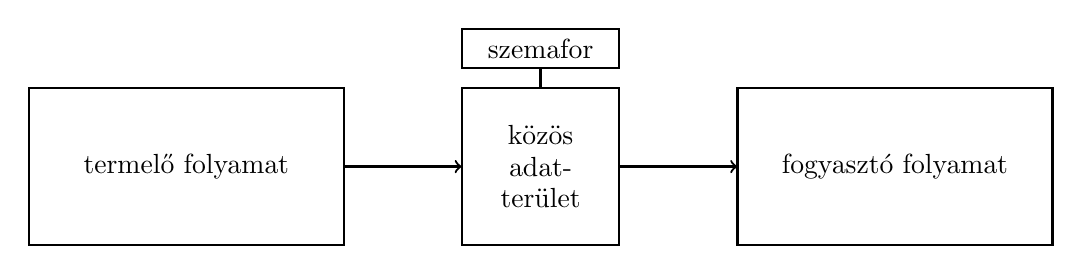
\begin{tikzpicture}
      \draw[thick] (0,0) rectangle ++(4,2);
      \node at (2,1) {\fkod{termelő} \fkod{folyamat}};
      
      \draw[thick] (5.5,0) rectangle ++(2,2);
      \node at (6.5, 1.4) {\fkod{közös}};
      \node at (6.5, 1) {\fkod{adat-}};
      \node at (6.5, 0.6) {\fkod{terület}};
      
      \draw[thick] (9,0) rectangle ++(4,2);
      \node at (11,1) {\fkod{fogyasztó} \fkod{folyamat}};
      
      \draw[thick] (5.5,2.25) rectangle ++(2,.5);
      \node at (6.5,2.5) {\fkod{szemafor}};
      
      \draw[->, thick] (4,1) -- (5.5,1);
      \draw[->, thick] (7.5,1) -- (9,1);
      \draw[thick] (6.5,2) -- (6.5,2.25);
      
      %\draw[implies-implies,double equal sign distance, semithick] (2,0) -- (2,-0.75);
      %\draw[implies-implies,double equal sign distance, semithick] (2,-1.5) -- (2,-2.25);
    \end{tikzpicture}
  \end{figure}
  
  Mielőtt a folyamat használni kezdené a közös erőforrást,
  ellenőriznie kell, hogy szabad-e. Csak akkor kezdheti el
  használni, ha a szemafor szabadot jelzett.
  A \zkod{primitív} megszakíthatatlan, oszthatatlan művelet.
  Legyen $P$ (\fkod{foglalttá állítás}) és $V$ (\fkod{szabaddá állítás})
  primitívek $\mathbf{S}$ bináris szemafor.

  \begin{figure}[H]
    \centering
    \begin{tikzpicture}
      \draw[
        rounded corners=10,
        color=bgreen,
        ultra thick
      ] (0,0) rectangle ++(7,4);
      \draw[
        rounded corners=10,
        color=bgreen,
        ultra thick
      ] (9,-1) rectangle ++(7,2);
      
      \draw[thick, ->] (12, 2.5) to [bend left=20](7,2) {};
      \draw[thick, ->] (7, 1) to [bend right=15](9,0) {};
      \draw[above] node at (12,2.5) {\zkod{primitív művelet}};
      
      \draw node[black, text width=6cm] at (3.5, 2.25){
        \begin{enumerate}[leftmargin=*]
          \item a szemafor olvasása
          \item beolvasott érték vizsgálata
          \item ha szabad: foglaltra állítás
          \item ha foglalt: vissza 1-re
        \end{enumerate}
      };
      \draw node[black, text width=6cm] at (12.5, 0.25){
        \begin{enumerate}[leftmargin=*]
           \setcounter{enumi}{4}
          \item az erőforrás olvasása
          \item szemafor szabadra áll
        \end{enumerate}
      };
      \draw[below] node at (4,-1) {
        $P(\mathbf{S})$ $\rightarrow$
        \fkod{memória írás/olvasás}
        $\rightarrow$ $V(\mathbf{S})$
      };
    \end{tikzpicture}
  \end{figure}
  
  
  \fogalom{Postaláda kezelés}
  A \zkod{postaláda} olyan közös adatterület,
  ahová egynél több üzenet írható.
  Kezelése hasonlít az előző problémához.
  A vezérléséhez 3 szemafor szükséges, $P$ és $V$ primitívek:
  \begin{itemize}
    \item $\mathbf{S}$ – a kölcsönös kizárást valósítja meg,
    bináris (\fkod{0-foglalt}, \fkod{1-szabad})

    \item $\mathbf{TELE}$ – a tele helyek száma, nem bináris,
    (értéke: \fkod{0\dots{}N}, kezdetben \fkod{0})

    \item $\text{\textbf{ÜRES}}$ – a tele helyek száma, nem bináris,
    (értéke: \fkod{0\dots{}N}, kezdetben \fkod{N})

    \item $P$ – szemafor értékét eggyel csökkenti (\fkod{foglalttá állítás})
    
    \item $V$ – szemafor értékét eggyel növeli (\fkod{szabaddá állítás})
  \end{itemize}

  \begin{figure}[H]
    \centering
    \begin{tikzpicture}
      \draw[thick] (0,0) rectangle ++(4,2);
      \node at (2,1) {\fkod{termelő} \fkod{folyamat}};
      
      \draw[thick] (5.5,0) rectangle ++(2,2);
      \node at (6.5, 1.4) {\fkod{közös}};
      \node at (6.5, 1) {\fkod{adat-}};
      \node at (6.5, 0.6) {\fkod{terület}};
      
      \draw[thick] (9,0) rectangle ++(4,2);
      \node at (11,1) {\fkod{fogyasztó} \fkod{folyamat}};
      
      \draw[thick] (5.5,2.25) rectangle ++(2,.5);
      \node at (6.5,2.5) {\fkod{$\mathbf{S}$}};
      \draw[thick] (6.5,2) -- (6.5,2.25);

      \draw[thick] (6.6,-0.75) rectangle ++(1.8,.5)
      node[midway] {$\text{\textbf{ÜRES}}$};
      \draw[thick] (7,-.25) -- (7,0);

      \draw[thick] (4.6,-0.75) rectangle ++(1.8,.5)
      node[midway] {$\text{\textbf{TELE}}$};
      \draw[thick] (6,-.25) -- (6,0);

      \draw[->, thick] (4,1) -- (5.5,1);
      \draw[->, thick] (7.5,1) -- (9,1);
      
      \draw[
        rounded corners=10,
        color=bgreen,
        ultra thick
      ] (0.5,-5) rectangle ++(3,4.5)
      node[black, text width=2.5cm, midway]{
        \begin{itemize}[leftmargin=*]
          \item $P(\text{\textbf{ÜRES}})$
          \item $P(\mathbf{S})$
          \item \fkod{mem írás}
          \item $V(\mathbf{S})$
          \item $V(\mathbf{TELE})$
          \vspace{0.5cm}
        \end{itemize}
      };

      \draw[
        rounded corners=10,
        color=bgreen,
        ultra thick
      ] (9.5,-5) rectangle ++(3,4.5)
      node[black, text width=2.5cm, midway]{
        \begin{itemize}[leftmargin=*]
          \item $P(\mathbf{TELE})$
          \item $P(\mathbf{S})$
          \item \fkod{mem írás}
          \item $V(\mathbf{S})$
          \item $V(\text{\textbf{ÜRES}})$
          \vspace{0.5cm}
        \end{itemize}
      };
    \end{tikzpicture}
  \end{figure}
  
  \fogalom{Szemaforok}
  A közös adatterületet egyszerre csak egy folyamat használhatja.
  (\zkod{kölcsönös kizárás}) A vezérlés \zkod{szemafor}ok
  segítségével történik. Lehetnek binárisak és nem binárisak.
  
  
  % ----------------------------------------------------------------------------
  % ------------------------------ Section 14 ----------------------------------
  % ----------------------------------------------------------------------------
  \section{Tétel – Az operációs rendszerek alapjai} %14
  

  \fogalom{Holtpont}
  lorem
  \fogalom{Holtpont kezelése}
  lorem
  \fogalom{Holtpont észlelése}
  lorem
  \fogalom{Holtpont megelőzés}
  lorem
  \fogalom{Bankár algoritmus}
  lorem


  % ----------------------------------------------------------------------------
  % ------------------------------ Section 15 ----------------------------------
  % ----------------------------------------------------------------------------
  \section{Tétel – Az operációs rendszerek alapjai} %15
  
  \fogalom{Ütemezési algoritmusok}
  lorem
  \fogalom{Előbb jött – előbb fut algoritmus}
  lorem
  \fogalom{A legrövidebb előnyben algoritmus}
  lorem
  \fogalom{Körbenforgó algoritmus}
  lorem
\end{document}